
\documentclass[conference]{IEEEtran}
\usepackage[utf8]{inputenc}
\usepackage[T1]{fontenc}

% *** CITATION PACKAGES ***

\usepackage{cite}





% *** GRAPHICS RELATED PACKAGES ***
%
\ifCLASSINFOpdf
  % \usepackage[pdftex]{graphicx}
  % declare the path(s) where your graphic files are
  % \graphicspath{{../pdf/}{../jpeg/}}
  % and their extensions so you won't have to specify these with
  % every instance of \includegraphics
  % \DeclareGraphicsExtensions{.pdf,.jpeg,.png}
\else
  % or other class option (dvipsone, dvipdf, if not using dvips). graphicx
  % will default to the driver specified in the system graphics.cfg if no
  % driver is specified.
  % \usepackage[dvips]{graphicx}
  % declare the path(s) where your graphic files are
  % \graphicspath{{../eps/}}
  % and their extensions so you won't have to specify these with
  % every instance of \includegraphics
  % \DeclareGraphicsExtensions{.eps}
\fi


%%%%IMAGE PACKAGE
\usepackage{graphicx}


\begin{document}

\title{
%Performance Factors for Large Scale Machine Learning Applications
Perfomance Factors of Deep Learning and Shallow Neural Network Applications: A Beginners Guide
}

\author{\IEEEauthorblockN{Johannes Wünsche}
\IEEEauthorblockA{Otto-von-Guericke University Magdeburg\\
johannes.wuensche@st.ovgu.de}
}

% make the title area
\maketitle

% As a general rule, do not put math, special symbols or citations
% in the abstract
\begin{abstract}

Machine Learning is probably the most present topic of computer science in general media. This popularity only increased over the recent years thorugh widely publicly known applications ranging from DeepBlue to IBM Watson and AlphaGo. Because of these successes Machine Learning, and the specialized sub-field of Deep Learning,  is sometimes viewed as an omnipotent solution to every imaginable problem. This is most certainly not the case. Based on our studies we can conclude that the capabilities of neural networks (i.e., the model used in deep learning) depend on the quality of their training. This process, in turn, can be time-consuming. Its performance depends on good design and engineering work. In this paper we want to give an short introduction into the most performance influencing factors when working with neural networks, with a focus on their training stage.
\end{abstract}

\IEEEpeerreviewmaketitle
\section{Introduction}
Machine Learning seems to be everywhere around us. With the recent success of Neural Networks, and other Machine Learning tools, especially  in general media well reported learners like AlphaGo or IBM Watson, these technologies are experiencing a kind of renaissance. Their usage has spread from industrial(e.g. self-driving cars, which rely on autonomous interpretation of camera feed and sensor output using machine learning) to retail. Also in modern automation and research, machine learning becomes a greater tool for managing to find more efficient ways to achieve better results in many cases.

In this paper we want to observe and identify the most performance influencing factors of these networks while designing and implementing them for specific applications, with both small and large scale deployments.
We expect that this study will provide help for readers interested in learning about the the initial design of neural networks, requirements for managing data, and operations of an efficient neural network.

During our research we found no comprehensive study touching this topic. The most closely related work are studies with a focus on comparing different platforms or frameworks. This paper is based on these publications.

 At first we attend to the choice of neural network and the impact of this decision. Afterwards we have a look, on one hand, at small scale neural networks running on a single machine without large data sets and on the other hand, large scale neural networks operating with more layers and nodes, large data sets and a distributed system to handle the computational power required by the neural network training algorithms to be completed in reasonable time. We divide our survey into
\begin{itemize}
\item the choice of neural network
\item the choice of processing units, including basic data distribution strategies for multi-processing
\item a discussion of the challenges in running small and large scales.
\end{itemize}

%%%%BEGIN RELATED WORK

The topic of considering the performance of neural networks and the influencing factors, has been covered in many studies like
 in "Benchmarking state-of-the-art deep learning software tools" \cite{shi2016benchmarking} and "Paleo: A performance model for deep neural networks" \cite{qi2016paleo}. In our study we hope to offer a collected view, which could serve as an entry point for developers seeking to work with these tools.
%%%%END RELATED WORK

%%%%%%%%%%%%%%%%%%%%%%%%%%%%%%%%%%%%%%%%%%%BEGIN BACKGROUND

\section{Background and Related Work}

\begin{figure}
\centering
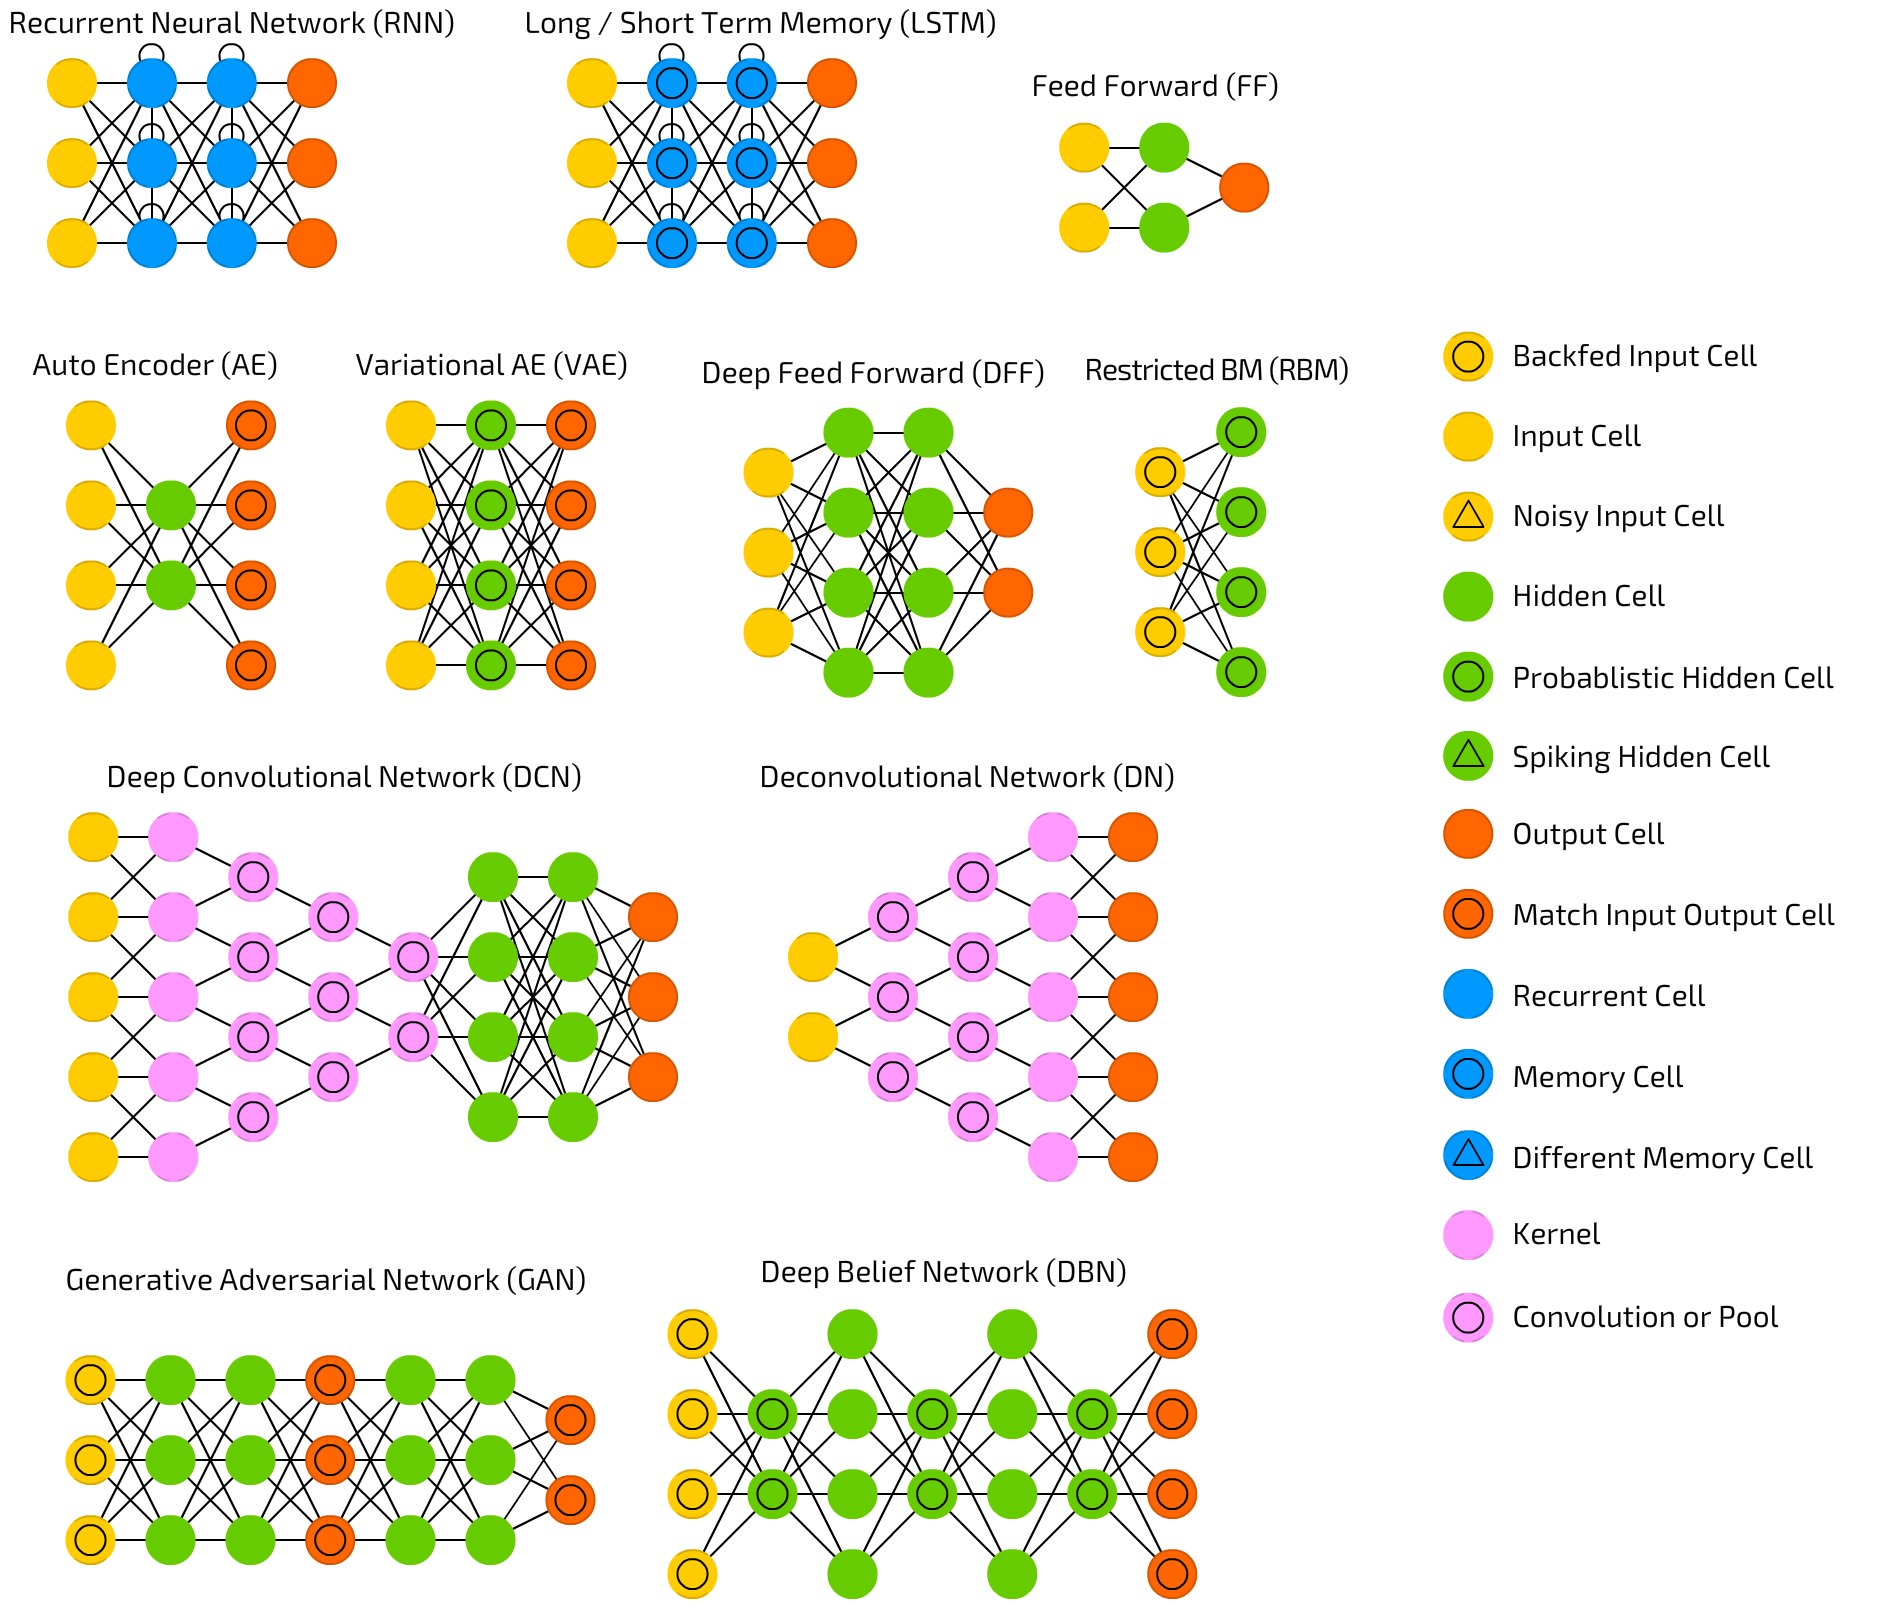
\includegraphics[width=0.5\textwidth]{neuralnetworks.png}
\caption{"A mostly complete chart of Neural Networks" by "The Asimov Institute" extract of only in this paper referenced networks\cite{zoo}}
\end{figure}


%%%%BEGIN DEEP LEARNING

In this section we introduce some commonly used models, we consider some performance factors and we refer readers to related work in evaluating performance factors of these models. For this we begin by showing some of the history of Deep Learning followed by clarification of the distinction between what we define as small and large scale networks.

The term "Deep Learning" itself is just a rebranding of the since the 50s existing concept of multilayered perceptrons\cite{frank1957perceptron}. Its basic idea is to simply use more than 1 layer in a neural network to increase the accuracy of the learned model\cite{deeplearning101}. A good defintion of Deep Learning is delivered by Deng in his 2014 book "Deep learning: methods and applications"\cite{deng2014deep}: "A class of machine learning techniques that exploit many layers of non-linear information processing for supervised or unsupervised feature extraction and transformation, and for pattern analysis and classification". Additionally to the reuse of multilayer perceptrons the ideas of Deep Belief Networks and unsupervised pretraining were introduced in 2006\cite{hinton2006fast}, opening the door for continuous improvements in different aspects of neural networks. Among the relatively recent developments in neural networks has been the adoption of GPUs for processing, as exemplified in work winning the ImageNet challenge\cite{krizhevsky2012imagenet}.

\begin{figure}
\centering
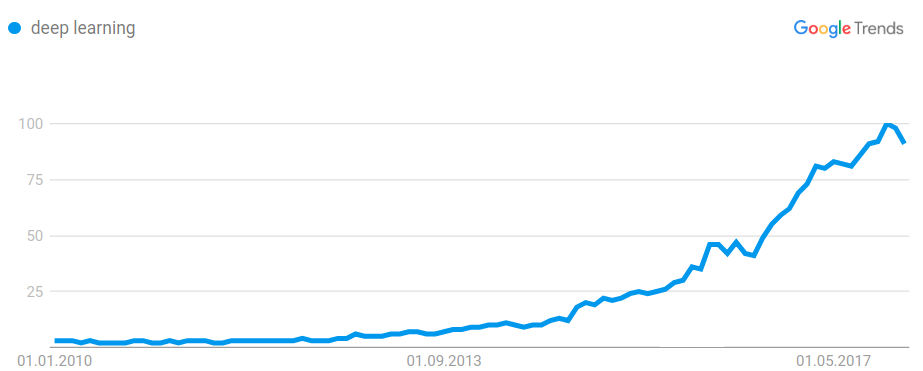
\includegraphics[width=0.5\textwidth]{pop.png}
\caption{Popularity in \% of the term "deep learning" on Google in relation to maximum peak, plotted with the Google Trends tool provided by Google}
\end{figure}


Since then Deep Learning has experienced an almost exponential growth in popularity as seen in Figure 2, where the popularity steeply increased around 2014.
%%%%END DEEP LEARNING

%%%%BEGIN SMALL SCALE NEURAL NET DESCRIPTION

As a small scale neural network applications we define a network with few and because of this rather limited size it. Most of the time such a network is run on a single machine.

%%%%END SMALL SCALE NEURAL NET DESCRIPTION

%%%%BEGIN LARGE SCALE NEURAL NET DESCRIPTION

On the other hand as a large scale neural network applications we define a network with a large number of nodes which can, because of the complexity of the resulting connections take a large amount of time to complete training if computed on one processing unit. Therefore it requires a system capable of running the training parallel in a single processing unit, a system containing multiple processors in one node, or a multinode system. Or in other words a system capable of parallelization, since this is of highest concern in large scale networks.
%%%%END  LARGE SCALE NEURAL NET DESCRIPTION

%%%%BEGIN DESCRIPTION NETWORKS USED LATER

%simple
The most commonly used shallow Neural Networks are Feed Forward, Auto Encoders and Restricted Boltzmann Machines, which all have only a single layer of hidden nodes and therefore are quite restricted in what they can compute based on the input data. They are shown in Figure 1.

Feed Forward Networks(FFN) simply connect input, hidden and output layers with an all to all connection between the layers with the number of outputs being equal or smaller to the number of hidden nodes.

Auto Encoders(AE) are of a similar build but the hidden layer compresses the input information into fewer nodes while these are later again decompressed to output nodes that match the previously given input nodes, therefore AE can be classified as a generative network.

Restricted Boltzmann Machines(RBM) only have an input and an output layer with an all to all connection between these. This RBM has in comparison to the normal Boltzmann Machine a better training behaviour which leads to a faster trained network.

%deep
A more advanced architecture is to increase the number of hidden layers to enlarge the application possibility of these networks for more complex models, these are then called Deep Networks. The more commonly used ones are Variational Auto Encoders , Deep Belief Networks, Generative Adversial Networks, Recurrent Neural Networks, e.g. Long short-term memory networks, Deep Convolutional Neural Networks, Deconvolutional Networks, and Recursive Neural Networks. They are also shown in Figure 1.

Variational Auto Encoders(VAE) consists of an encoder, sampler and decoder and are able to to generate output based on specification given to the VAE. 

Deep Belief Networks(DBN) are a combination of RBM and FFN in which the RBM are used to pretrain the network with the initial training 
data and the FFN to adjust the learned values slightly to improve the result. The pretraining is done in an unsupervised manner enabling the network to learn structural features of the input in each layer. These networks are at the core of the renaissance of neural networks, stemming from the work of Hinton 2006\cite{hinton2006fast}.

Generative Adversial Networks(GAN) like the VAE create random output based on the model found in the given training data. VAE are a specialization of GAN because of the restrictions that can be set for the output which is not possible in a GAN.

Deep Convolutional Networks(DCN) are based on Convolutional Nodes compressing the incoming information into the needed base model and then calculating the required output\cite{PattersonGibson17}. They are used to abstract input information into more general models. These networks are specially being used to process images.

Deconvolutional Networks(DN)\cite{zeiler2014visualizing} are less surprisingly the opposite of DCN in the idea that input information is first spread to a larger amount of nodes and then processed by the following Nodes to be used by the output.

Long short-term memory(LSTM)\cite{hochreiter1997long} are a variant of Recurrent Neural Networks(RNN) including additionally memory cells and gates that control the content of the cells, that are able to remember patterns in sequential data. This model has been able to improve learning process of RNN and results.

%%%%END DESCRIPTION NETWORKS USED LATER

%%%%BEGIN TRAINING ALGORITHMS
%%THE POSITION OF THIS CAN BE CHANGED
The reason why the training of neural networks is so expensive can be traced back to the algorithm used to train all commonly used networks, which is backpropagation. Backpropagation is based on the idea that we first calculate the deviation of the output values from the actual result and then use this backwards thorugh the layers of the net to calculate a correction,based on the error of the node and the learning rate, for each connection weight until the input layer is reached\cite{riedmiller1993direct}. Some Networks like DBN use a slightly 
different "Gentle" Backpropagation, which relies on a learning rate after the initial values have been found from the training data with the help of the pretrained RBM \cite{PattersonGibson17}.
%%%%END TRAINING ALGORITHMS

%%%%BEGIN INFORMATION DATA FLOW

Another performance influencing factor besides the actual neural net and the learning algorithm, is the amount of data required for the net to be trained and the size of each training example.While this is mostly important for large scale applications, it can also be hindering for smaller ones. For example if we use a Convolutional Neural Network to classify the content of a greyscale picture we get for small $512*512$ sized images $262144$ inputs that each need to be transferred to the processing unit, CPU or GPU, for each example.

This large amount of data can, for one, take some time to be transferred, if for example this data package is required by an external processing unit like a GPU other units cannot receive new data and therefore the performance drops due to them being idle. Also if too much data is needed in relation to the actual output the data storage can achieve enduring performance loss will occur.  

Furthermore if the training data exceeds the memory for the processing unit, the problem of delivering data to all units becomes more pressing.

%%%%END INFORMATION DATA FLOW

%%%%BEGIN PROCESSING UNIT

The next major performance influencing factor will be the choice of the actual processing unit. This decision is the most computation time influencing. This decision can have the biggest influence on computation time. We divide our processing unit into three groups starting with the CPUs, which have a greater memory capability because they can be equipped with additional RAM sticks but possess a smaller parallelization limitation than GPUs because of their different architecture, then the GPUs,with a much larger architectural focus on multithreading than CPUs, and following GPU-Clusters, being simply a group of GPUs either in a single node or spanning multiple nodes, like they are used in supercomputers.

%%%%END PROCESSIONG UNIT

%%%%BEGIN INFORMATION ACTUAL USED IMPLEMENTATIONS

The most common neural network frameworks which we, because of their wide popularity, have found in performance studies are Tensorflow\cite{abadi2016tensorflow}, Caffe\cite{jia2014caffe}, Torch\cite{collobert2002torch}, CNTK\cite{gitcntk}, deeplearning4j\cite{websitedl4j}, Keras\cite{websitekeras}, and MXNET\cite{websitemxnet}.

% These frameworks have been benchmarked in numerous settings and applications and can help us show performance influencing factors.

%TODO some more detailed stuff about it
%%%%END INFORMATION ACUTAL USED IMPLEMENTATIONS




%Transition
Next will follow the choice of neural netwok as well as the setting of some hyper-parameters like the amount of nodes, followed by the choice of the processing unit


%%%%%%%%%%%%%%%%%%%%%%%%%%%%%%%%%%%%%%%%%%%%%%%%%%%%BEGIN CHOICE OF NETWORK

\section{Performance impacting choices}	

%%%%BEGIN IMPORTANCE
The first important choice is to what neural network is going to be used. This decision is heaviliy reliant on the application that is to be implemented. Such decision influences all further actions and has to be carefully made.

To assist this decision we offer some general guidelines for when to use shallow vs. deep networks, and what specializations of certain networks could be advantageous for specific tasks.
%%%%END IMPORTANCE

%%%%BEGIN ADVANTAGES DISADVANTAGES SIMPLE AND DEEP
\subsection{Choice of Neural Network}
\subsubsection{Shallow Networks}
Simple learning task can be done by a network which is not deep, like a FFN or a RBM. They are faster to train and even larger training sets can be completed in a reasonable time without multithreading or usage of GPUs. But their limited depth can decrease the accuracy of the model when the learned task is more complex than expected. In other words, these models have a risk to overfit the training data. Accordingly, to use them, careful validation is required. 

\subsubsection{Deep Networks}
More complex tasks often require a deep neural network that can learn a more complex model than shallow networks and offer a greater accuracy while doing this. The major downside of these networks is that they require a larger amount of time to train and can be oversized for the actual learning task, adding unnecessary computation time. Large scale applications mostly contain deep networks because of their larger training sets and more complex models underlying the actual task.

We can not offer a clear answer about when to use which kind of network. Every problem must be individually analyzed and based on the information, and complexity, as well as the acceptable error rate of the final network the decision has to be made. For cases that are unclear a shallow network can first be constructed,because of their short training time, and if the result is unsatisfying a more complex network can be considered.  Also it is advisable to use a deep network if the learning task involves image or audio understanding, or the task needs to include recurring changes over time of an input signal\cite{PattersonGibson17}.
%%%%END ADVANTAGES DISADVANTAGES SIMPLE AND DEEP

%%%%INTITAL VALUES

Initial values, next to the number of nodes, the type of network, the activation functions, the activation thresholds, learning rate, the size of the batches, the training algorithm, the number of training epochs, and others, are called the hyper-parameters of the network. We can define these, informally, as the configurable factors that determine the training process in the network and the convergence of error rates. In our discussion, (given that our focus is on performance, with a data management perspective) we only consider the number of nodes. The precise effect of other hyper-parameters is, arguably less data management related, and thus, beyond the scope of our work.

%%%%END INITIAL VALUES

%%%%DETAILS SIMPLE AKA SMALL
\subsection{Shallow network node amount}
If a shallow network shall be used the next choice will be the amount of nodes in the hidden layer. This is of course dependent on the number of inputs and outputs. The number of hidden notes should not deviate too strongly from these two. The amount of the deviation is really dependent on the chosen neural network, for example a feed forward network profits when the number is equal or larger than the number of inputs, while an auto encoder probably has fewer hidden nodes. When the number of nodes is higher than the optimum, there can be a loss of accuracy or an increase in the number of epochs needed for training. In general this effect can be larger for deep networks than for shallow ones.

%%%%END DETAILS SIMPLE AKA SMALL

%%%%DETAILS DEEP AKA LARGE AND SMALL
\subsection{Deep networks node amount}
Like in shallow networks the amount of nodes to be used is an important value that determines the final ability of the network to fulfill its task in the required accuracy and speed. The actual number of nodes chosen at the end is of course a bit more complex in deep networks. For example networks like DCN require a special node configuration based on their basic idea(step by step decreasing of nodes per layer until desired compression reached) , or DN(opposite of DCN). So how the node configuration looks like is strongly dependent on the net chosen and the training task.

%%%%END DETAILS DEEP AKA LARGE AND SMALL

%%%%SPECIFIC NETS

\subsection{Specific deep networks}
Based on the content of the task a few networks can be more fitting than others to fulfill it. To deliver a short overview of it we use a classification by Patterson\cite{PattersonGibson17}.

%generation
If the task includes the generation of data a GAN, VAE or RNN/LSTM is recommended. Which of these to choose is strongly dependent of the specific parameters of the task. For example if we want to generate random new data following the model of our training data, the closest to this would be a GAN because it is by design built to fulfill such tasks. But if new data which is not completely random is to be generated a VAE can be considered which offers by design this possibility. In practice there are lots of generation examples available using these networks for example image generation with GAN\cite{junyanz2017} (For the interested reader, we suggest \cite{zhu2016generative} as a paper describing this approach) or text generation with LSTM\cite{gittesttensorflow} (Described in \cite{sutskever2011generating}).

%classification
If the task includes classification or interpretation of visual data deep neural networks, like CNN or DBN, can be used. For once CNNs are a straightforward choice since they are able to compress data and therefore abstract smaller data like the content of an image from the original image. But DBN also offer a possibility to complete the task with the major advantage of being able to first roughly guess values based on the training data and then train unsupervised in the fine-tuning phase as shown by Zhong 2016\cite{zhong2016diversified}.

%sequential data
If the task includes the classification or intepretation of incoming data over time the ability of RNN and LSTMs to remember data comes in handy. For example voice recognition is possible to implement with the help of LSTMs as shown by Soltau 2016\cite{soltau2016neural}.
%%%%END SPECIFIC NETS

Finally, if the task has been covered in the literature, it is worthwhile to use existing publically available networks like AlexNet, GoogleNet and others.

%Transition
To further optimize training time we will next touch the topic of processing units which can be used.



%%%%%%%%%%%%%%%%%%%%%%%%%%%%%%%%%%%%%%%%%%%%%%%%%%%%%BEGIN CHOICE OF PROCESSING UNIT


\subsection{Choice of Processing Units}
The next important choice is the choice of the processing units. We distinguish them into three main models, CPU, GPU, Multi-GPU and GPU-Clustering. In this section we discuss how these units can be used for deep learning. We base our discussion on published results of experiments \cite{shi2016benchmarking} and \cite{sastre2017scalability}. 


\subsection{CPU}
As the first most naive option we have a look on the CPU for training the neural net with either a simple single thread, or the more complex multi-thread.


\subsubsection{Single-thread}
The most naive implementation is the single-thread CPU calculation. Because of its sequential execution and calculation, it can be the slowest (when not taking into account the use of vectorized instructions). For networks with a large number of nodes this approach is simply unfeasible because of the excessive calculation time. Since this approach does not utilize the full capacity of the CPU, it can result in performance losses when compared to multi-threaded solutions (Table I).


\subsubsection{Multi-thread}
A more complex approach consists of utilizing the multi-core characterisitics of modern CPUs, by parallelizing the calculations in the training that only depend on previously calculated values. This is for example preferrable when training with the help of a \emph{Backpropagation} algorithm. As researchers observe, the benefits continue to grows by using more threads but reaches its limits when using more threads than physical cores available.

\begin{table} 
\centering
\begin{tabular}{c c c c c}
\hline
Framework & 1 Thread & 2 Threads &4 Threads & 8 Threads\\\hline
Caffe & 1.324 & 0.790 & 0.578 & 15.444 \\
Tensorflow & 7.062 & 4.789 & 2.648 & 1.938 \\
Torch & 1.329 & 0.710 & 0.423 & na \\\hline
\end{tabular}
\caption{Training time(in s) for a mini-batch of size 64 of a Fully Connected Network(FCN) trained with synthetic data on a i7-3820 with 4-physical cores using 3 different commonly used Deep Learning frameworks\cite{shi2016benchmarking}}
\label{fig_ttfcn}
\end{table}

%limit
Though this approach is limited by the actual core number available and should not overstep the number of physical cores, like with \emph{hyper-threading} technologies, which can lengthen the required calculation time because of a more inefficient usage of the CPU\cite{shi2016benchmarking}.


\subsection{GPU}
A more advanced implementation is to use the shared memory, multi-core environment of modern GPUs. For example with the help of  NVIDIAs CUDA this can be done efficiently and results in a speed-up of deep learning algorithms of up to 3 times when compared to CPU-based approaches. Almost all deep learning frameworks support GPUs. 
%restrictions
Problems lie in the tightly restricted memory of graphic cards that may not be able to contain all nodes with their corresponding weights.  Furthermore there might be some communication overhead between CPUs and GPUs, since the latter can have a higher throughput, and there might be an imbalance making the communication of data and results a bottleneck. Accordingly, one solution, the overlapping of computation of communication is an important technique.


\subsection{Multi-GPU}
To further improve performance during training multiple GPUs can be used to train the neural net. This shortens training time but also requires new actions like synchronizations of GPUs and splitting of data and/or neural network.

%speedup numbers
A main advantage of Multi-GPU is of course the increased computation power available during the training phase, reducing training time by 35\% when doubling the number of GPUs in CNTK and MXNET, 28 \% in Caffe and 10 \% in  Torch and Tensorflow\cite{shi2016benchmarking}.

%memory
Another advantage is the greater availability of memory somewhat easing the restrictions of the memory restricted GPUs structure. While this is an advantage it is not efficient if used as the single goal of multiple GPU usage because of the high price connected to acquiring them.

\begin{figure}
\centering
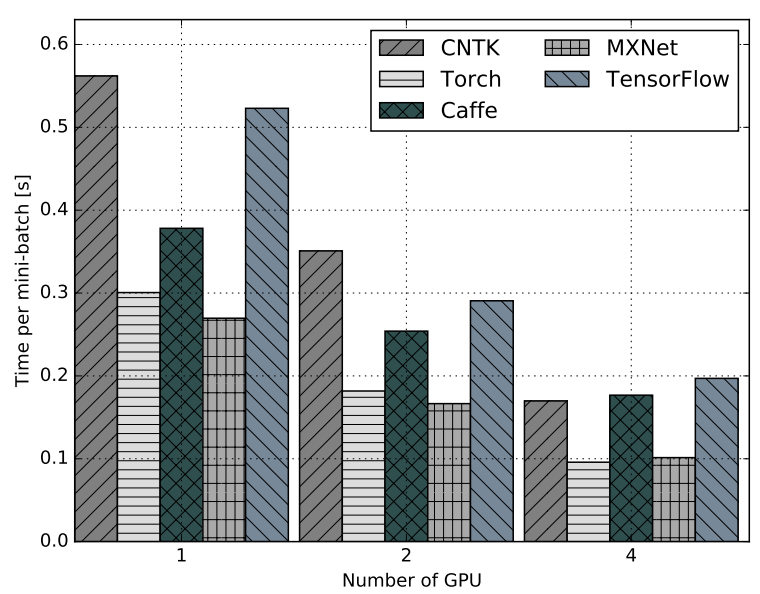
\includegraphics[width=0.4\textwidth]{a.png}

\caption{Time per mini-batch in s compared between different amount of GPUs used\cite{shi2016benchmarking}}
\label{fig_m_gpu}
\end{figure}

%speedup figure
Figure 3 visualizes this improvement showing the reduction of training time steadily with the increasing of amount of GPUs. Although costly this leads to a constant improvement. Higher Numbers of GPUs can be again slower or offer no significant improvement if used in a single system because of an increasing communication overhead and bottleneck for the data flow in the CPU, which is responsible for managing separate GPUs.

\subsubsection{Parallelism between GPUs}
There are two kind of parallelism approaches applicable to the problem, first there is data parallelism which splits the training data into multiple sets. Each subset and a complete replica of the model is assigned to a processing unit, such that each can calculate the gradients for all the layers. Finally, before moving to the next epoch, the gradients of all units are aggregates such that the parameters can be updated, shipping a new replica for the next epoch. This can be done by dividing the data by case or by feature. The second approach is model parallelism in which the net is divided into separately runnable parts, each part can be assigned to a separate unit such that all units train over the complete data, but each calculates gradients for a subset of neural network nodes. Naturally, inter-processing unit communication might be needed when the gradients have to be propagated to other processors. For networks that do not have fully connected layers, such that the distribution can be made avoiding (to an extent) inter-unit processing. This method is also fitting for single node distributions in which the GPUs share one PCIe bus, but lead to the result being more vulnerable to calculation failures \cite{sastre2017scalability}.

\subsubsection{Synchronization between GPUs}
For synchronizing Multi-GPU setups like in Figure 5 there are theoretically two choices. One being the synchronous method in which after a value is calculated it is immediately shared with every other GPU. This method is applicable to all Multi-GPU configurations and delivers an acceptable result\cite{wang2016deep}. The update of values for all GPUs occurs only after the updated values have been sent by each of them. Until a large amount of over 40 GPUs are used this mehtod can be used without limitation\cite{sastre2017scalability}. 
There is also the possibility to run the GPUs asynchronously, by letting them use different versions of the values and only updating them periodically by sending an update request. This can lead to a slight improvement of the training speed but it might also have a slight detrimental effect in the learning process\cite{wang2016deep}. This depends on the network model and training algorithm. 




\subsection{GPU-Clusters}

The next logical step is to use multiple Multi-GPU systems further reducing training time but also creating new challenges, because of the decentralized nature of the Cluster, like communication overhead.  This is mostly used in large scale applications and is most of the time not needed in small scale.

\begin{figure}
\centering
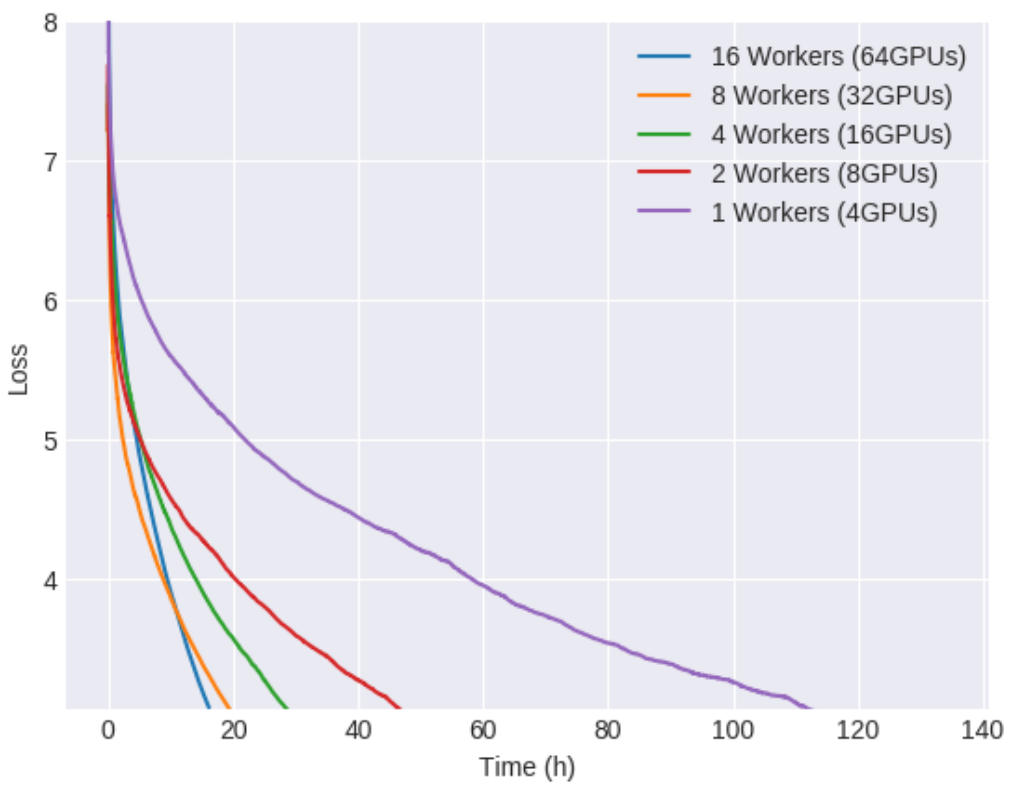
\includegraphics[width=0.4\textwidth]{gpu_cluster_perf_win.png}
\caption{Time (in h) of different asynchronous configurations until reaching destined error rate(loss)\cite{sastre2017scalability}}
\label{fig_cl_gpus}
\end{figure}

\subsubsection{Multiple GPU-Clusters}
Taking a step further it is possible to connect multiple Clusters of GPUs to compute a single task. In doing this we again increase raw computation power, but also increase the total amount of communication required. Similar to multiple GPUs this leads at the beginning with 2 or more Clusters to a stronger improvement than later on with 8 to 16 Clusters as seen in (Figure 4)

\subsubsection{Parallelism of multiple GPU-Clusters}
Like the Multi-GPU setup this can be done by creating either data or model parallelism. Combination are also possible, for instance in a setup consisting of multiple Clusters and one single communication server model parallelism can be used to distribute the model on the different clusters, but they internally can use data parallelism to split the work\cite{wang2016deep}.

\subsubsection{Synchronization of multiple GPU-Clusters}
The synchronization of GPU-Clusters can be undertaken either with synchronous or asynchronous approaches. These tactics can also be combined to create a mixed-asynchronous strategy, using an asynchronus training on inter-cluster level and on intra-cluster level synchronous training\cite{sastre2017scalability}. This approach is specially reasonable considering that intra-cluster communication will usually be much faster than inter-cluster communication. This creates the best performance on large configurations with many clusters\cite{wang2016deep}. Which challenges this and other characteristics of this incur will be explained in the next section.

%%%%%%%%%%%%%%%%%%%%%%%%%%%%%%%%%%%%%%%%%%%%%%%%%BEGIN CHALLENGES


\section{Large scale challenges and Small scale challenges}
Different scales of deep learning models have different challenges that need to be considered during the design and implementation of the neural network.

\subsection{Small scale challenges}
First and foremost it is important to notice that the biggest restrictions of small scale applications is the limited computation power available during the initial training process, later during the usage of the net for inference (also called prediction serving), this is less impactful because either the net is completely pretrained and not changed later or the changes are limit like some optimization when the network receives a query.

%model choice
This leads to the focus lying on the design to find the best fit of complexity to fit the desired model. Otherwise longer training time or less accuracy of the resulting network will occur.

%rest trivial
Further small scale applications are relatively free of performance related complications, because of their relative simplicity and fast modern computer hardware.

\subsection{Large scale challenges}
In contrast to small scale applications, the most challenging factor for large scale applications is the proper scheduling of operators, to reduce the costly communication and synchronization between processing units. This problem occurs because a larger data flow has to be managed over more processing units compared to small scale applications.

\begin{figure}
\centering
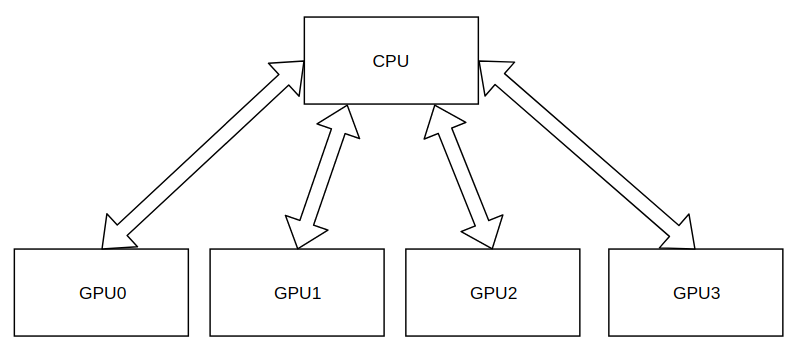
\includegraphics[width=0.4\textwidth]{example_configuration.png}
\caption{One example configuration consisting of a CPU and 4 connected GPU units for training the neural network.}
\end{figure}

%%Data flow of training data
The \emph{data flow} is a problem on multiple fronts.On one side the transfer of the training data from main memory to GPU memory can be the first bottleneck restricting faster processing speeds from being realized. For example if the GPU only receives data and no calculation is currently active this slows down the training process unnecessarily. To increase the speed of the calculation data can be fetched during the processing of already present data, this is called data prefetching as described and implemented by Yang 2010 \cite{yang2010gpgpu}. This solution can solve the problem partially but reaches its limits when used with multiple GPUs. For example configuration (Fig. 3), this makes the CPU-GPU transfer the single bottleneck, if the data for an iteration (training data plus the model) in each individual GPU is too large to fit in the GPU memory. For example a GPU equipped with PCI-Express 4.0 with a x16 Throughput can at best receive 31.5 GB/s, if we assume that all training data can reside in the CPU main memory, that way if we need to refresh the complete memory of a modern GPU like NVIDIA GTX 1080, we need 0.253968 s, so to refresh all GPUs memory without including any overhead produced by switching operations between the GPUs we have an absolute transfer time of 1.015873 s, and for 3 units 0.7619 s, so if our GPU completes the desired calculation faster, for example 0.5 s, we have a 0.2619 s period in which our GPU is idle every iteration. Therefore we have an effective calculation computation time each phase of 65.62 \%. This problem only grows if the main memory is too small to fit the complete training data since connections to solid state disk are too slow and hard disk do physically do not reach the required throughput.

%%data flow synchronization
Additional data flow is created when \emph{synchronizing GPUs} with each other, by approaches described beforehand in "Choice of Processing Units", they each have their own advantage but can limit efficiency in certain situations. Both create an communication overhead because during transmission of values the GPU cannot operate on the neural network training.

\begin{figure}
\centering
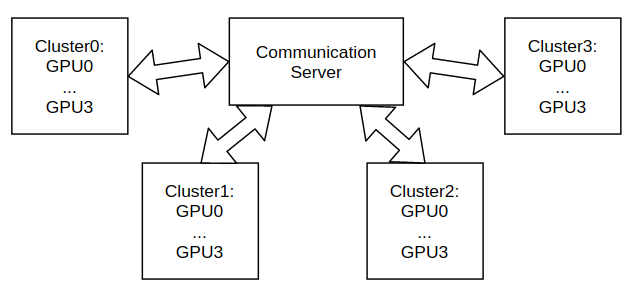
\includegraphics[width=0.4\textwidth]{cluster_setup.png}
\caption{One example configuration consisting of a communication server and 4 connected GPU-Clusters each containing 4 GPUs.}
\end{figure}
%synchronous
Synchronous training, while being recommend for setups that have 40 GPUs or less, can create idle time if one unit is slower than others, since all updates have to be sent to the server before the next iteration can be undertaken, this slows down all other units. This problem becomes more likely the more units are used. Also more GPUs lead to more communication if synchronization is required after very step, so they increase the amount of data managed by the CPU or communication server. This applies to configurations like Figure 5 and Figure 6.

%asynchronous
If an \emph{asynchronous training} approach is used problems may occur influencing the result, if updates are too sporadic and different versions of values drift too far apart. To avoid this problem GPU-Cluster configurations do not rely on complete asynchronous training startegies, but on the already described mixed-asynchronous approach, minimizing this problem while still reducing possible communication overhead.

To ease the effect of \emph{GPU to GPU communication},by relieveing the CPU of managing them, technologies like GPUDirect from NVIDIA\cite{nvidiagpudirect2017} can be used allowing direct GPU to GPU communication if they are connected to the same PCIe bus, so this is only appplicable within a GPU-Cluster or a single system and does not remove all communication overhead. Also shared memory between GPUs can be useful, reducing synchronization between them (and enabling, to an extent, model parallelism cross GPUs)

%memory limitation
\emph{Memory limitation} is another issue appears while training if the training data is too large to fit in memory. Then time expensive disk accesses to either very slow HDDs or faster but still relatively slow SSDs are required. For example a fast available SSD SAMSUNG 960 PRO can reach up to 3.5 GB/s which is still relatively slow compared to the maximum 31.5 GB/s possible through an PCIe x16 interface. To further increase speed a RAID 0 setup can be created consisting of multiple M.2 SSDs with the potential of parallel access and data transfer reaching for instance with 5 960 PRO that could transfer at maximum of around 17 GB/s.

%bandwith between clusters
\emph{Cluster communication} becomes only more and more concerning when more GPU-Clusters are used, because the connection between them may be slower than the interfaces of RAM, GPU and storage used therefore creating a new bottleneck. This problem can be reduced if training data is stored by the cluster, which has the downside of further increasing the cost of these setups.


%%%%%%%%%%%%%%%%%%%%%%%%%%%%%%%%%%%%%%%%%%%%%%%%%BEGIN CONCLUSION


\section{Conclusion}
%Summary
During our survey we observed that the most influencing factors are the basic choice of neural network to be used, this includes its complexity as well as the actual architecture of the network is build of. Furthermore the processing unit that is chosen has a strong influence on the quality and speed of training the network. Based on the choice of this other factors came into consideration influencing the process, like communication between processing units and parallelism of data between them. They are not quite as influential as the first two but can lead to a strong improvement or worsening. We observed that even in example systems that handle communication efficiently about 35 \% of the calculation time is sacrificed to it, as in our example previously.

%Takeaway
Especially data transfer time and alike carries a potential to lengthen the training time to a significant amount. To ease this, technologies like GPUDirect\cite{nvidiagpudirect2017} and data prefetching\cite{yang2010gpgpu} can be used. It may be possible to decrease the effect of the data flow further by introducing a direct memory transfer unit which can indepently organize synchronization and can handle parallel transfers to and from multiple GPUs. This could decrease the calculation time to a bare minimum but would require additional hardware and maybe modification of the used GPUs. Although this could break some security limits because of unauthorized memory accesses. 

%End
In the end, these are factors that need to be considered by both data scientist working with networks, and systems developers who build deep learning systems. Considering the benefits of these technologies, we believe that more research on improving these runtimes could be beneficial. As future work we suggest that edge computation for networks (a pertinent topic for Intelligent Personal Assistants like Google Now, Siri or Alexa) should also be studied more by system developers.

% use section* for acknowledgment
\section*{Acknowledgment}
The author would like to thank Gabriel Campero Durand for advise and help to write the paper


% trigger a \newpage just before the given reference
% number - used to balance the columns on the last page
% adjust value as needed - may need to be readjusted if
% the document is modified later
%\IEEEtriggeratref{8}
% The "triggered" command can be changed if desired:
%\IEEEtriggercmd{\enlargethispage{-5in}}

\bibliographystyle{IEEEtran}
\bibliography{paper}


% that's all folks
\end{document}


